\documentclass[tikz,border=2pt]{standalone}
\usepackage{amsmath}
\usepackage{amssymb}
\usetikzlibrary{arrows.meta}
\begin{document}
% Closed three-station network: from station 1 a job goes to 2 (prob 0.6) or 3 (prob 0.4), and
% both return to 1. Visit ratios V=(1,0.6,0.4) solve V=VP with V_1=1; with E[S]=(1,1.5,2) the
% work per cycle V_i E[S_i]=(1,0.9,0.8) is largest at station 1, the bottleneck.
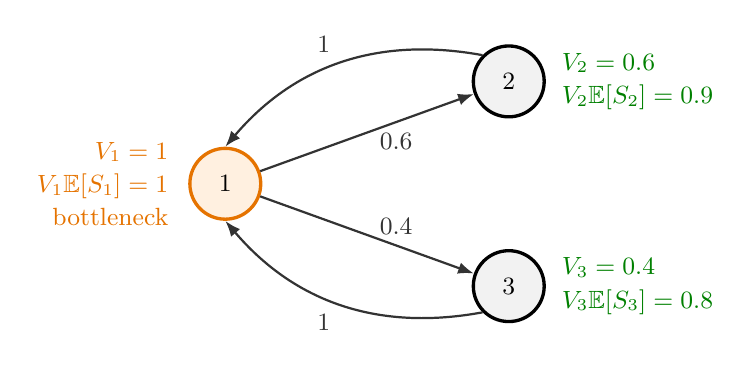
\begin{tikzpicture}[font=\small, >={Latex[length=2mm]},
  st/.style={circle, draw=black, very thick, fill=gray!10, minimum size=9mm}]
  \node[st, draw=orange!90!black, fill=orange!12] (s1) at (0,0) {$1$};
  \node[st] (s2) at (3.6,1.3) {$2$};
  \node[st] (s3) at (3.6,-1.3) {$3$};
  \draw[->, thick, gray!40!black] (s1) -- node[below right, pos=0.55, xshift=-3pt, yshift=2pt] {$0.6$} (s2);
  \draw[->, thick, gray!40!black] (s1) -- node[above right, pos=0.55, xshift=-3pt, yshift=-2pt] {$0.4$} (s3);
  \draw[->, thick, gray!40!black] (s2.north west) to[bend right=30] node[above left] {$1$} (s1.north);
  \draw[->, thick, gray!40!black] (s3.south west) to[bend left=30] node[below left] {$1$} (s1.south);
  % visit ratios and work per cycle
  \node[anchor=east, align=right, orange!90!black] at (-0.6,0) {$V_1=1$\\[1pt] $V_1\mathbb{E}[S_1]=1$\\[1pt] bottleneck};
  \node[anchor=west, align=left, green!50!black] at (4.15,1.3) {$V_2=0.6$\\[1pt] $V_2\mathbb{E}[S_2]=0.9$};
  \node[anchor=west, align=left, green!50!black] at (4.15,-1.3) {$V_3=0.4$\\[1pt] $V_3\mathbb{E}[S_3]=0.8$};
\end{tikzpicture}
\end{document}
